\documentclass{article}


\usepackage{amsmath} % math stuff
\usepackage{amssymb} % math stuff
\usepackage{array} % equations and stuff
\usepackage{bm} % bold math
%\usepackage{caption} % suppressed table numbering; incompatible with revtex, and longtable, I think
\usepackage{comment} % comment environment
%\usepackage{enumitem} % customization of enumeration, itemize, and description
\usepackage[T1]{fontenc} % font encoding for special characters, must also use scalable font package
\usepackage[margin=0.8in]{geometry} % paper sizes and margins (but be careful not to mess up pre-defined pages)
\usepackage{graphicx} % for graphics
%\usepackage{helvet} % default font is the helvetica postscript font
\usepackage{lipsum} % lorem ipsum filler text
\usepackage{lmodern} % scalable font?
\usepackage{longtable} % multi-page tables
\usepackage{mathrsfs} % math script font
\usepackage{mhchem} % easier chemical formula
\usepackage{microtype} % allows disabling of ligatures
%\usepackage{newcent} % new century schoolbook font
\usepackage{nicefrac}
\usepackage{parskip} % removes paragraph indentation, and adjusts paragraph skip, as well as list items
%\usepackage{setspace} % adjust text spacing and indents
\usepackage{siunitx} % decimal alignment
\usepackage{subfigure} % divided figures
%\usepackage{tabu} % extra table options
\usepackage{textcomp} % symbols
\usepackage{threeparttablex} % better footnotes with longtable
\usepackage{titling} % title placement
\usepackage{ulem} % strikethrough text
%\usepackage{url} % superceded by hyperref
\usepackage{verbatim} % verbatim environment
\usepackage{xcolor} % colors and color boxes
\usepackage{xspace} % commands that don't eat up white space
\usepackage{hyperref} % links and page setup; should always come last

\hypersetup{
	bookmarks=true,
	colorlinks=true,
	citecolor=blue,
	linkcolor=blue,
	urlcolor=blue,
	pdfstartview={XYZ null null 1.0} % default open view is 100%
}

\DisableLigatures[f]{encoding = *, family = * } % disable ff, fi, fl ligatures, without f option, it also disables -- = endash
\renewcommand{\arraystretch}{1} % extra vertical space in tables

\begin{document}

\pagestyle{empty} % don't number pages

% custom title
\begin{center}
{\LARGE Classic Riddler}

\vspace{0.15in}

{\Large 5 June 2020}
\end{center}


\section*{Riddle:}

Some friends have invited you to a protest, and you'll be making a sign with large lettering.
You're filling in the sign's letters by drawing horizontal lines with a marker.
The marker has a flat circular tip with a radius of 1 centimeter, and you're holding the marker so that it's upright, perpendicular to the sign.

Since the diameter of the marker's tip is 2 centimeters, you decide to fill in the letters by drawing lines every 2 centimeters.
However, this is the pattern you get:

\begin{center}
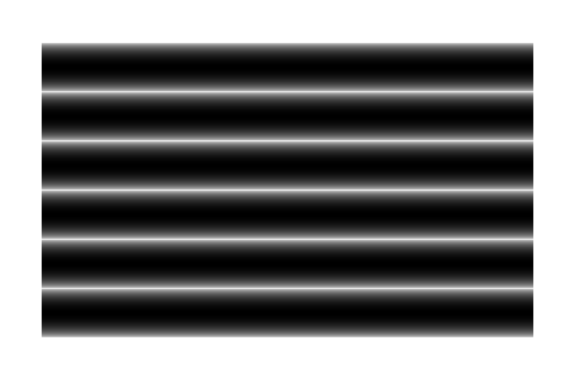
\includegraphics[width=3in]{poster.png}
\end{center}

The shading doesn't look very uniform---each stroke is indeed 2 centimeters wide, but there appear to be gaps between the strokes.
Of course, if you drew many, many lines all bunched together, you'd have a rather uniform shading.

But you don't have all day to make this sign.
If the lines can't overlap by more than 1 centimeter---half the diameter of the marker tip---what should this overlap be, in order to achieve a shading that's as uniform as possible?
And how uniform will this shading be, say, as measured by the standard deviation in relative ink on the sign?

\section*{Solution:}

This was a tricky problem.
The idea is that each stroke of the marker produces a line that varies in thickness (``shading'' in the riddle) according to the cross-sectional width of the marker.
By making some of the strokes overlap, there are now regions where the thickness is the sum of the widths from the bottom and top of the marker.
But of course, if the stroke separation is anything more than 1~cm, there are also regions with just a single stroke's thickness.
The problem is the find the ideal stroke separation so that the thickness across both the single- and double-stroke regions stays as uniform as possible.
The uniformity will be measured by the standard deviation of the thickness.

To solve this problem, I considered the thickness only between the centers of two strokes.
The rest of the drawing will just be a repeated version of this.
The region I considered will have one part only from the bottom part of the first stroke, a part with overlap, and a part from the top of the second stroke.
The functional form of the individual stroke thicknesses are circles.

I will let the first stroke be centered at $x=0$, and the second stroke at $x=1+d$, with $0\leq d\leq1$ so that the strokes are separated by at least 1, but still have overlap.
I will call the functions of the individual strokes $g_{1}(x)$ and $g_{2}(x)$ so that their sum is $g(x)$.
The functions are:
\[
g_{1}(x)=\sqrt{1-x^{2}}\ ,
\]
\[
g_{2}(x)=\sqrt{1-(x-(1+d))^{2}}\ ,
\]
\[
g(x)=
\begin{cases}
g_{1}(x) & 0\leq x<d \\
g_{1}(x)+g_{2}(x) & d\leq x<1 \\
g_{2}(x) & 1\leq x\leq1+d \\
\end{cases}
\ .
\]

The problem is to find $d$ which minimizes the standard deviation of $g(x)$ across the region from 0 to $1+d$.
But it's not clear how to get the standard deviation of $g(x)$, since it is not a probability density function.
Luckily, I in my research, I ran across the Law of the Unconscious Statistician.
This states that if the probability distribution of a function $g(x)$ is not known, then its expectation value can still be calculated if the probability distribution of $x$ is known.
In this case, $x$ is distributed uniformly in the region above, so its probability distribution is
\[
f(x)=
\begin{cases}
\frac{1}{1+d} & 0\leq x\leq1 \\
0 & \text{elsewhere}
\end{cases}
.
\]
To get the standard deviation, I will need to calculate both two expectation values: the mean and variance.
The law says that the expectation value (mean) $\mu$ is simply given by
\[
\mu=\text{E}[g(x)]=\int g(x)f(x)\ dx\ .
\]
Similarly, the variance is given by
\[
\text{E}\left[(g(x)-\mu)^{2}\right]=\text{E}\left[g(x)^{2}\right]-\mu^{2}\ .
\]

The mean is easy to calculate, since it is just the integral of the two stroke functions.
Because the functions are just quarter circles, each area is simply $\nicefrac{\pi}{4}$, so the mean is $\mu=\nicefrac{\pi}{2+2d}$.

The variance is quite a bit harder to calculate.
The expectation of $g(x)^{2}$ becomes
\[
\text{E}\left[g(x)^{2}\right]=\frac{1}{1+d}\int_{0}^{d}g_{1}(x)^{2}\ dx
+\frac{1}{1+d}\int_{d}^{1}\left(g_{1}(x)+g_{2}(x)\right)^{2}\ dx
+\frac{1}{1+d}\int_{1}^{1+d}g_{2}(x)^{2}\ dx\ .
\]
For my calculations, I labeled the terms $I_{1}$, $I_{2}$, and $I_{3}$, so that
\[
I_{1}=\frac{1}{1+d}\int_{0}^{d}1-x^{2}\ dx\ ,
\]
\[
I_{2}=\frac{1}{1+d}\int_{d}^{1}\left(\sqrt{1-x^{2}}+\sqrt{1-(x-(1+d))^{2}}\right)^2\ dx\ ,
\]
\[
I_{3}=\frac{1}{1+d}\int_{1}^{1+d}1-(x-(1+d))^{2}\ dx\ .
\]

The first and last term are equal due to symmetry, and have value
\[
I_{1}=I{3}=\frac{d-\nicefrac{1}{3}d^{3}}{1+d}\ .
\]

The second term is much harder.
I again divided up the integral:
\begin{align*}
I_{2} &=\frac{1}{1+d}\int_{d}^{1}1-x^{2}+1-(x-(1+d))^{2}\ dx
+\frac{2}{1+d}\int_{d}^{1}\sqrt{1-x^{2}}\sqrt{1-(x-(1+d))^{2}}\ dx \\
&=I_{4}+I_{5}\ .
\end{align*}
I'm sure that the last term has an analytical solution, but it would have way to many terms to try to deal with.

The goal of the riddle is to minimize the standard deviation, but this is equivalent to minimizing the variance.
So that's what I chose to do: minimize the variance, then calculate the standard deviation after.
Even if the variance is known analytically, calculating the minimum requires a derivative, which trying to set to 0 would be impossible analytically.
Therefore, any solver would have to come up with a numerical answer.
So I might as well just solve the variance itself numerically, and obtain the minimum by observation.

\vspace{0.5in}

That's what I did in the spreadsheet \texttt{numeric\_stdev.xlsx}\,.
I calculated the mean and each integral of the variance for several values of $d$, and focused in on the minimum values.
The resulting plot of the standard deviation looks like this:

\begin{center}
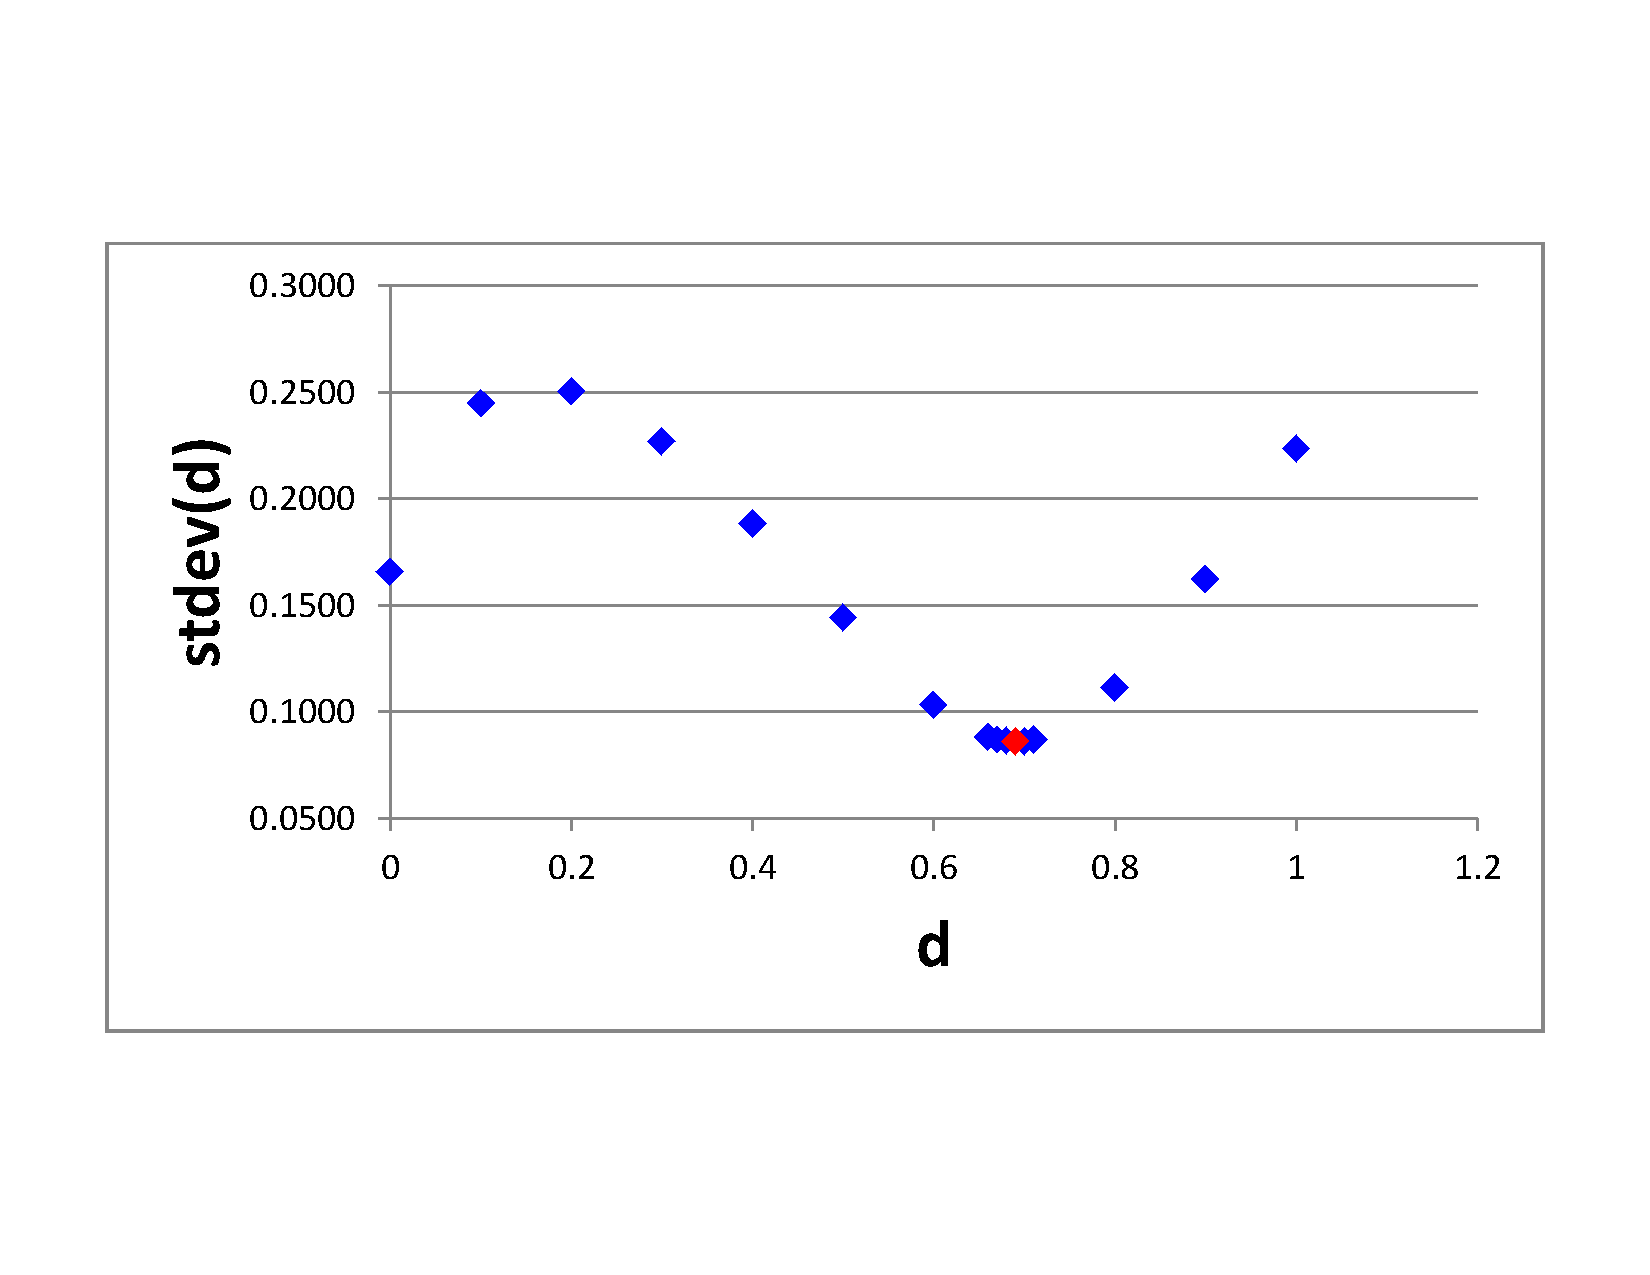
\includegraphics[clip, trim=0in 1in 0in 1in, width=4in]{numeric_stdev_chart.pdf}
\end{center}

The ideal marker separation is therefore
\fcolorbox{red}{white}{\bf d=1.69}
which produces a normalized thickness of
\fcolorbox{red}{white}{$\bm{92.9\pm8.6\%}$}\,.
I will note here that my solution does not consider any saturation effects---that is, I did not set a maximum value for $g(x)$.
That means that in this calculation, two overlapping marker strokes can become more shaded than the thickest single stroke.
Ultimately, then, there's really no concept of being completely black; any other stroke could always make a region more shaded.

So what does this actually look like?
I have drawn a plot of the thickness/shading as a function of the distance between the two marker centers below, although I have not produced an improved version of the first image.
That's a bit too much for me.

\begin{center}
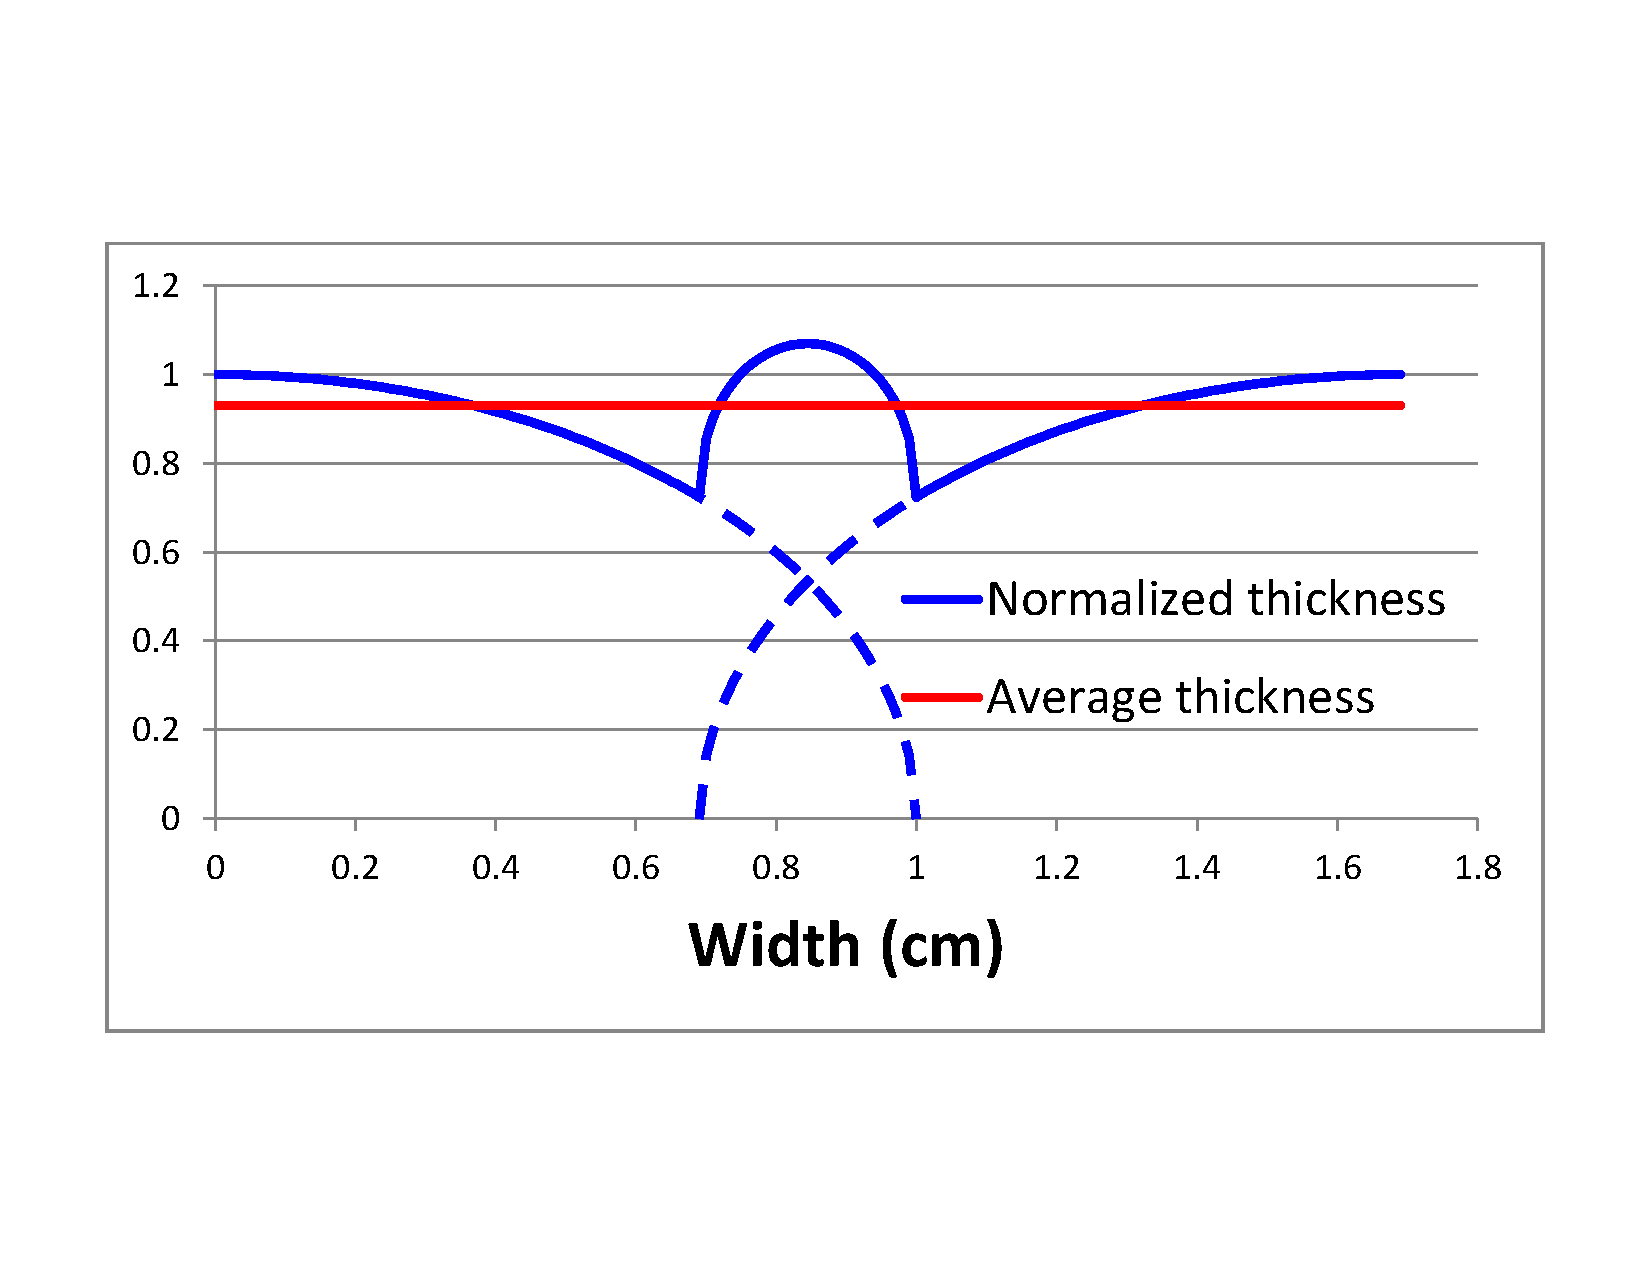
\includegraphics[clip, trim=0in 1in 0in 1in, width=4in]{thickness.pdf}
\end{center}




\end{document}